\chapter{True Polymorphic Phase Transition or Dynamic Crystal Disorder? An Investigation into the Unusual Phase Behavior of Barbituric Acid Dihydrate} 
The following chapter contains published work written by me with the guidance of Dr. Matthew King. This work is published at Ref. \citep{paul_true_2019}. 
\label{chap:BTADH}
\section{Abstract}
Crystalline barbituric acid dihydrate (BTADH) was previously thought to undergo a subtle temperature-dependent phase transition from a high-temperature orthorhombic \textit{Pnma} space group to a non-merohedrally twinned monoclinic \textit{P}2\textsubscript{1}/\textit{n} phase below a transition temperature of ~217 K. Questions remain on the true nature of the unusual transformation and the structure of the high-temperature crystal phase due to difficulties in resolving the \textit{Pnma} structure from X-ray diffraction data and because of the subtlety of the structural transition. In this study, terahertz (THz) spectroscopy and solid-state density functional theory (DFT) were utilized to explore this suspected phase transition and uncover the principle physical mechanisms contributing to this anomalous transition. Our findings suggest that at temperatures above the previously reported phase transition temperature of 217 K, the crystal does not exist in the \textit{Pnma} space group configuration. However, two equivalent favorable energetic states with \textit{P}2\textsubscript{1}/\textit{n} symmetry related by the twinning plane lie on either side of the proposed \textit{Pnma} structure. It is these same local potential energy minima that guide the crystal system to a non-merohedrally twinned configuration identified in the low-temperature crystal structures. At temperatures above 217 K, the system possesses the thermal energy necessary to readily transition between these degenerate states separated by the low-lying \textit{Pnma} structural barrier. The evidence acquired by THz spectroscopy and DFT indicate the absence of a true temperature-dependent phase change, and rather a system that exists in a tenuous thermally disordered state above the previously alleged transition temperature.
\section{Introduction}

The crystalline conformation of compounds can have a large influence on material properties, such as solubility, dissolution rate, melting point, and mechanical properties, and these can vary significantly between polymorphs of a compound \citep{Brittain2016,bernstein_polymorphism_2011,gentili_polymorphism_2019}. As polymorphism has a profound influence on such physicochemical properties, the study of the growth and transformation of polymorphs and solvatomorphs have become a quite impactful area of interest for pharmaceutical development, crystal engineering, and de novo materials design\citep{galindo_control_2017,maini_chemical_2015,hiremath_controlling_2005,cocca_influence_2011,lee_crystal_2011,moulton_molecules_2001,baskar_raj_pseudo-polymorphism_2003}. However, detailed experimental and computational analyses of complex target systems can often be difficult. In ongoing efforts to improve computational methodologies to describe the behavioral intricacies of crystal systems, it is useful to accompany such approaches with experimental spectroscopic analyses in the study of polymorphism, phase transitions, and related phenomena.
In this study, solid-state density functional theory (DFT) and terahertz (THz) spectroscopy were used to explore the underlying physical mechanisms leading to a subtle temperature-dependent phase transition exhibited by the barbituric acid dihydrate (BTADH) crystal system. THz spectroscopy has been shown to be a powerful tool for the investigation of molecular crystals and polymorphism since THz radiation can be used to probe phonon vibrations sensitive to the specific intermolecular interactions present in a particular molecular packing configuration \citep{ruggiero_resolving_2016,ruggiero_predicting_2018,king_understanding_2011,king_identification_2011,delaney_understanding_2012}. In combination with DFT calculations, valuable information can be obtained regarding structure, energetics, and vibrational properties \citep{ruggiero_concomitant_2017,allis_solid-state_2006}. 
Crystalline BTADH is reported to undergo a transition from a high-temperature orthorhombic \textit{Pnma} phase to a non-merohedrally twinned monoclinic \textit{P}2\textsubscript{1}/\textit{n} phase below a transition temperature of ~217 K (\autoref{BTADH_fig}). The BTADH system has been extensively studied by X-ray diffraction, with most attempts at resolving the high-temperature phase resulting in the investigators reluctantly coming to the same conclusions. The most thorough study was performed by Nichol and Clegg in 2005, whom measured the BTADH system at 14 temperatures ranging from 100–270 K, with meticulous focus on temperatures surrounding the suspected transition temperature reported at 216–217 K \citep{nichol_btadh_2005}. Most unusual is the subtlety of the phase transformation undergoing no changes in hydrogen bonding motifs upon the \textit{Pnma} to \textit{P}2\textsubscript{1}/\textit{n} transition, only an out-of-plane rotation of the barbituric acid molecules and modest displacements of the two H\textsubscript{2}O molecules and the sp3-hybridized carbon of barbituric acid. The authors ultimately determined a high-temperature \textit{Pnma} phase, which was in line with two preceding studies also proposing the \textit{Pnma} space group at room temperature \citep{1961_Jeffrey,1977_Al-Karaghouli}. These studies reported quite large atomic displacements along the b-axis, perpendicular to the mirror plane containing all atoms, besides the mirrored sp3 hydrogens. Furthermore, Al-Karaghouli et al. studied the BTADH system by neutron diffraction and proposed that the crystal may take a Pn21a configuration or that the H\textsubscript{2}O oxygen atoms may not lie within the mirror plane \citep{1977_Al-Karaghouli}. However, neither proposition gave satisfactory results, leading both studies to settle on the \textit{Pnma} space group assignment. All previous reports do agree that the BTADH crystal system at temperatures below 217 K adopts the \textit{P}2\textsubscript{1}/\textit{n} space group and exhibits non-merohedral twinning relating equivalent \textit{P}2\textsubscript{1}/\textit{n} unit cells by a two-fold rotation about the b-axis. 

\begin{figure}[ht]
  \center
  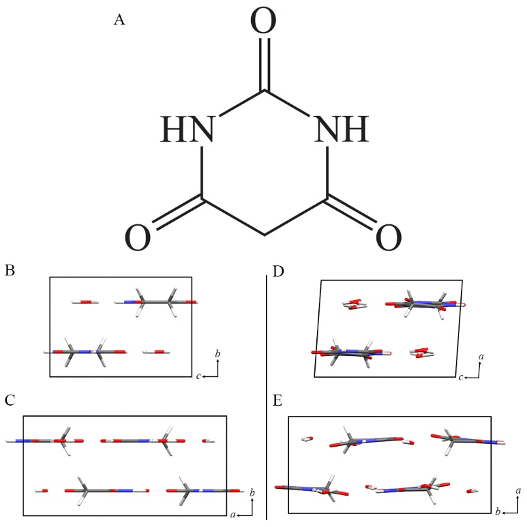
\includegraphics[width=7.5cm]{src/figures/btadh_figs/btadh_fig1.png}
  \caption{A) Molecular structure of barbituric acid. Comparison of the crystalline structures of the temperature-dependent BTADH polymorphs, with the high-temperature \textit{Pnma} form viewed along the B) a-axis and C) c-axis, and the low-temperature \textit{P}2\textsubscript{1}/\textit{n} form along the D) b-axis and E) c-axis.}
  \label{BTADH_fig}
\end{figure}


\section{\nobreak Experimental Section}
\subsection{THz Spectroscopy}
Anhydrous barbituric acid (BTA) was obtained from Sigma-Aldrich (99\% purity). BTADH was crystallized from a saturated aqueous solution by slow evaporation at room temperature over a period of one week under darkness. Samples for THz measurements were mixed with polytetrafluoroethylene (PTFE) powder at concentrations of approximately 4.5\% by mass. The samples were pulverized using a stainless steel amalgamator (Dentsply Rinn 3110-3A) to minimize particle size and scattering of THz radiation. Approximately 0.50 g of the sample mixtures were pressed into pellets under a measured pressure of 2000 psi using a hydraulic press (ICL EZ-Press 12) equipped with a 13 mm stainless steel die. PTFE pellets for use as reference blanks were prepared in the same manner. THz spectra were recorded using a custom time-domain pulsed THz spectrometer based on an amplified Ti:sapphire laser system (Coherent, Inc., Santa Clara, CA), described in detail elsewhere \citep{rexrode_effects_2019}. Data were acquired at 293 and 78 K with samples under vacuum. Samples and blanks were scanned 32 times and data were averaged for each individual data set. Each 32-ps scan window consisted of 3200 data points representing the THz waveform, producing an effective instrument resolution was approximately 1.0 cm\textsuperscript{-1}. The ratio of the power spectra obtained from the Fourier-transformed data sets of the sample and blank produced the THz absorption spectrum. Each THz spectrum presented in this work is the average of four individual THz spectra.

\subsection{Solid-State Density Functional Theory}

All calculations were performed using the Crystal14 software package \citep{Dovesi2014,Dovesi2017}. Solid-state DFT calculations utilized the PBE,\citep{perdew} M06,\citep{zhao_m06_2008} and B3LYP \citep{Lee_1988,becke_density-functional_1993} functionals with atom-centered cc-pVDZ,\cite{dunning_gaussian_1989} 6-31G(d,p),\citep{hehre_selfconsistent_1972,Hariharan1973TheIO} 6-311G(d,p),\citep{krishnan_self-consistent_1980} and pob-TZVP \citep{peintinger_consistent_2013} basis sets. Initial lattice dimensions and atomic coordinates were acquired from X-ray crystallographic data from Cambridge Crystallographic Database\citep{nichol_btadh_2005,groom_cambridge_2016}. The sampling rate as a function of k points used in defining the real space density matrix and Monkhorst grid in reciprocal space was determined for total energy convergence criteria of \(\Delta\)E \(<\) 10\textsuperscript{-8} hartree for geometry optimizations and \(\Delta\)E \(<\) 10\textsuperscript{-11} hartree for normal-mode calculations \citep{gilat_analysis_1972,monkhorst}. In order to meet these convergence criteria, shrinking factors of 6 where used for the BTADH crystal calculations. The total number of grid points varied between calculations depending on initial crystal geometry. The radial and angular distributions of points were defined by a pruned (75,974) integration grid for each calculation. A pair-wise (D2) damped empirical energy correction for London-type dispersion forces as proposed by Grimme et al \citep{grimme_accurate_2004,grimme_semiempirical_2006}. was included in all DFT calculations. The global scaling factors, s6, used for the dispersion correction term were 0.75, 0.25, and 1.05 for PBE, M06, and B3LYP, respectively \citep{zhao_m06_2008,grimme_accurate_2004,grimme_semiempirical_2006,Karton_2009}. Additional dispersion parameters, including C6 coefficients, van der Waals radii, cut-off distance, and dampening function steepness, were taken from Grimme et al \citep{grimme_accurate_2004,grimme_semiempirical_2006}. Modifications to van der Waals radii were made in accordance with Civalleri et al. \citep{civalleri_b3lyp_2008}. for the application of D2 dispersion corrections in molecular crystals. The truncation tolerances for the Coulomb and HF exchange integral series are defined by the program keyword TOLINTEG, and were set to values of 10\textsuperscript{-8}, 10\textsuperscript{-8}, 10\textsuperscript{-8}, 10\textsuperscript{-8}, and 10\textsuperscript{-16} hartree. Frequencies of normal modes were calculated within the harmonic approximation by numerical differentiation of the analytical gradient of the potential energy with respect to atomic position\citep{pascale_calculation_2004}. The IR intensities for normal modes were calculated from the dipole moment derivatives (d$\mu$/dQ) determined by the Berry phase approach of calculating Born charges as polarization differences between equilibrium and distorted geometries \citep{zicovichwilson_calculation_2004}.

\section{Results and Discussion}
An initial screening of density functional and basis set combinations was performed to determine those best suited to reproduce the experimental X-ray crystal structures of BTADH by solid-state DFT. The PBE, M06, and B3LYP density functionals were employed, representing GGA, meta-GGA, and hybrid classes of functionals, respectively. Each density functional was combined with two different commonly used double-\(\zeta\) basis sets – 6-31G(d,p) and cc-pVDZ – and two triple-\(\zeta\) basis sets – 6-311G(d,p) and pob-TZVP. Geometry optimizations were performed in both fixed lattice dimensions of the 100-K structure and full-cell optimizations allowing lattice parameters to freely optimize within the constraints of space group symmetry. The 100-K X-ray crystal structure in \textit{P}2\textsubscript{1}/\textit{n} was used as the starting point for all calculations. \textit{Pnma} unit cells of the high-temperature crystal phase were not used for this initial evaluation as the crystal structures in \textit{Pnma} symmetry confine the BTA and H\textsubscript{2}O molecular orientations to planar configurations, thus no valuable information into functional/basis set performance can be obtained regarding intermolecular interactions from such calculations. The quality of structural reproduction was based on the notable structural variations presented through the suspected temperature-dependent phase transition using the series of BTADH crystal structures over the temperature range of 100–270 K reported in Ref. 18. For the geometry optimizations in fixed lattice dimensions, the angle between molecular planes between BTA molecules within a unit cell, the deviation of the CH\textsubscript{2} group from the BTA molecular plane, and the angle of planes formed by each of the two water molecules in the dihydrate asymmetric unit were used as metrics for structural reproduction (\autoref{btadh_planeorientations}). For full-geometry optimizations, lattice parameters a, b, c, and \(\beta\) were evaluated in addition to the aforementioned conformational metrics. These data for the experimental X-ray structures are provided in \autoref{btadh_latticeparams}.

\begin{figure}
  \center
  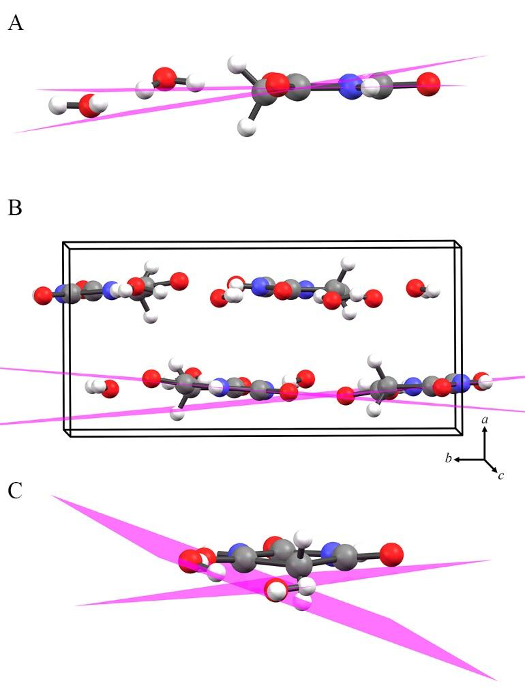
\includegraphics[width=7.5cm]{src/figures/btadh_figs/btdah_fig2.png}
  \caption{Plane orientations relating angle metrics for determining the quality of unit cell reproductions. A) BTADH molecular plane defined by ring carbonyl carbons, and that representing out-of-plane position of the ring CH\textsubscript{2} group. B) Opposing molecular planes of two symmetry-related BTADH molecules in the low-temperature \textit{P}2\textsubscript{1}/\textit{n} polymorph. C) Planes each created by a single H\textsubscript{2}O molecule of the dihydrate asymmetric unit.}
  \label{btadh_planeorientations}
\end{figure}

\begin{table}[ht]
  \centering
  \tiny
  \caption{Lattice parameters and calculated relative molecular orientations from BTADH experimental X-ray crystal structures reported in Ref. \citep{nichol_btadh_2005}.}
    \begin{tabular}{cccccccccc}
    \multicolumn{10}{l}{\textbf{Experimental X-ray}} \\
    \hline
    & \textbf{Space}  & & & & & & \textbf{CH\textsubscript{2}-} & \textbf{Mol-Mol} & \textbf{H\textsubscript{2}O-}\\
    \textbf{T (K)} & \textbf{Group} &	\textbf{a (Å)} & \textbf{b (Å)} & \textbf{c (Å)} & \textbf{\(\beta\)(°)} & \textbf{V (Å\textsuperscript{3})} & \textbf{Mol (°)\textsuperscript{a}} & \textbf{(°)\textsuperscript{b}} &	\textbf{H\textsubscript{2}O (°)\textsuperscript{c}} \\
    
    270 & \textit{Pnma}  & 6.2144 & 12.7512 & 8.8841 & 90 & 703.99 & -- & -- & -- \\
    230 & \textit{Pnma}  & 6.1739 & 12.7594 & 8.8831 & 90 & 699.77 & -- & -- & -- \\
    220 & \textit{Pnma}  & 6.1665 & 12.7630 & 8.8814 & 90 & 699.00 & -- & -- & -- \\
    219 & \textit{Pnma}  & 6.1624 & 12.7570 & 8.8780 & 90 & 697.90 & -- & -- & -- \\
    218 & \textit{Pnma}  & 6.1626 & 12.7570 & 8.8760 & 90 & 697.80 & -- & -- & -- \\
    217 & \textit{Pnma}  & 6.1770 & 12.7850 & 8.8980 & 90 & 702.70 & -- & -- & -- \\
    216 & \textit{P}2\textsubscript{1}/\textit{n} & 6.1567 & 12.7330 & 8.8650 & 91.180 & 694.80 & 1.85 & 2.98 & 28.87 \\
    215 & \textit{P}2\textsubscript{1}/\textit{n} & 6.1580 & 12.7514 & 8.8763 & 91.263 & 696.83 & 2.47 & 2.97 & 8.85 \\
    210 & \textit{P}2\textsubscript{1}/\textit{n} & 6.1538 & 12.7470 & 8.8770 & 91.627 & 696.00 & 2.85 & 3.6 & 20.31 \\
    200 & \textit{P}2\textsubscript{1}/\textit{n} & 6.1313 & 12.7030 & 8.8456 & 92.187 & 688.50 & 3.72 & 5.11 & 26.94 \\
    190 & \textit{P}2\textsubscript{1}/\textit{n} & 6.1377 & 12.7306 & 8.8641 & 92.528 & 691.94 & 4.81 & 5.9 & 16.72 \\
    170 & \textit{P}2\textsubscript{1}/\textit{n} & 6.1270 & 12.7253 & 8.8633 & 93.068 & 690.06 & 5.8 & 7.18 & 20.06 \\
    150 & \textit{P}2\textsubscript{1}/\textit{n} & 6.1130 & 12.7149 & 8.8564 & 93.437 & 687.14 & 6.7 & 8.22 & 25.09 \\
    100 & \textit{P}2\textsubscript{1}/\textit{n} & 6.0970 & 12.7152 & 8.8587 & 94.051 & 685.05 & 8.14 & 9.96 & 27.36 \\
    \hline
    \multicolumn{10}{l}{\textbf{DFT Full-Cell Geometry Optimizations in P2\textsubscript{1}/n}} \\
    & & & & & & & \textbf{CH\textsubscript{2}-} & \textbf{Mol-Mol} & \textbf{H\textsubscript{2}O-}\\
     \multicolumn{2}{c}{} &	\textbf{a (Å)} & \textbf{b (Å)} & \textbf{c (Å)} & \textbf{\(\beta\)(°)} & \textbf{V (Å\textsuperscript{3})} & \textbf{Mol (°)\textsuperscript{a}} & \textbf{(°)\textsuperscript{b}} &	\textbf{H\textsubscript{2}O (°)\textsuperscript{c}} \\
    \multicolumn{2}{c}{PBE/6-311G(d,p)} & 5.9263 & 12.6285 & 8.7625 & 94.455 & 653.81 & 8.76 & 10.53 & 24.04 \\
    \multicolumn{2}{c}{PBE/pob-TZVP} & 6.0755 & 12.4857 & 8.6603 & 94.438 & 654.97 & 11.39 & 15.53 & 40.25 \\
    \hline
    \multicolumn{10}{l}{\textsuperscript{a}CH\textsubscript{2}-Molecule planes (Fig. 2A); \textsuperscript{b}Molecule-molecule planes (Fig. 2B); \textsuperscript{c}Water-water planes (Fig. 2C).}
    \label{btadh_latticeparams}
    \end{tabular}
    \end{table}


It was determined from the extensive series of DFT structural calculations that the PBE density function in conjunction with the tested triple-\(\zeta\) basis sets, 6-311G(d,p) or pob-TZVP, were best suited for the computational treatment of the BTADH crystal system. The results of the computational screening are provided as \textbf{Supporting Information}. All subsequent calculations in this study utilized PBE/6-311G(d,p) and PBE/pob-TZVP. Results of the full unit cell geometry optimization using these functional/basis set combinations are also provided in \textbf{\autoref{btadh_latticeparams}}.
THz spectra of BTADH in the range of 20–95 cm\textsuperscript{-1} were obtained at 293 K and 78 K (\autoref{btadh_thz}A). Notable differences are present between the spectra taken at the two temperatures. At room-temperature, there is an absence of definitive spectral features below the one resolved peak at 88.8 cm\textsuperscript{-1}. Upon cooling to 78 K, six additional features emerge in the THz spectrum. Most conspicuous is the relatively narrow peak appearing at 33.6 cm\textsuperscript{-1} for which no evidence of any corresponding absorption intensity is present at 293 K. Large changes between THz spectra collected at different temperatures are usually indicative of a phase transformation leading to the activation/deactivation of phonon modes corresponding to the distinctive crystalline phases. In this case, however, there is not clear evidence of a phase transition between 293 and 78 K as many similarities remain between the two spectra, although many modes seem to be washed out at room temperature. There is an indication of underlying modes across the 293 K spectrum as broad absorptions resulting in a mostly featureless background that become resolved at low temperature. There is also a clear shift in the 88.8 cm\textsuperscript{-1} feature at 293 K to higher frequency upon cooling, which is typically observed temperature-dependent behavior for phonon modes.

\begin{figure}[h!]
  \center
  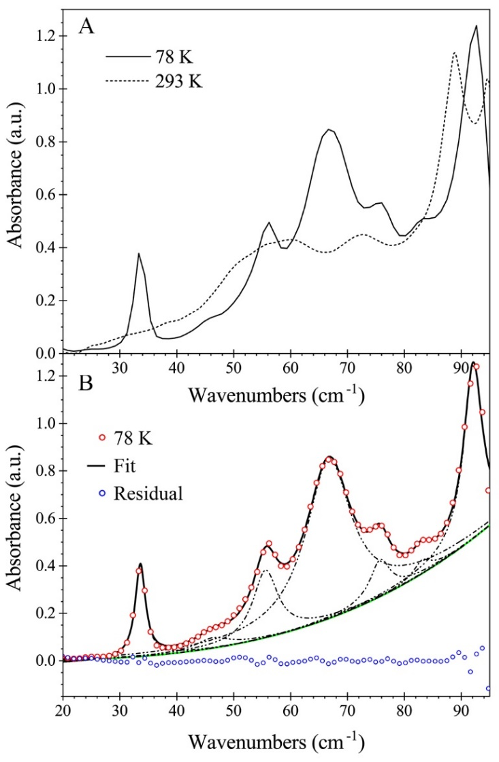
\includegraphics[width=6.5cm]{src/figures/btadh_figs/btadh_fig3.png}
  \caption{A) THz vibrational spectra of BTADH in the spectral range of 20-95 cm\textsuperscript{-1} obtained at 293 K and 78 K. B) Spectral fitting of the 78 K THz spectrum (red circles) with Lorentzian peaks (dashed lines) on exponential background (green line). The residuals of the experimental data and fitted values are indicated by blue circles.}
  \label{btadh_thz}
\end{figure}
\newpage
Another peculiar observance in the BTADH THz spectra collected at 78 K are the extremely broad symmetric absorptions between 40 and 80 cm\textsuperscript{-1}, and the discrepancy between linewidths of all present spectral features. A multiple peak fitting procedure was performed to determine the FWHM of the absorptions. Lorentzian line shapes for the seven distinguishable features were added to an exponential function representing the rising background, which is a product of Mie and Rayleigh scattering of THz radiation from the granular polycrystalline sample \citep{shen_elimination_2008}. The Lorentzian peaks and background were simultaneously fit to the experimental spectrum (\autoref{btadh_thz}B). Peak centers and FWHMs are provided in \autoref{thz_peaks}. The exponential function of form I=A\(\upsilon\)\^b , where I is the scattering intensity, A is the scalar accounting for particle size distribution, and b is the exponential factor influencing the frequency-dependence of scattering, yielded optimal values of A = 1.7 × 10\textsuperscript{-7} and b = 3.34. This value of b is in accordance with previously reported values using the same exponential form to correct for scattering effects observed in THz spectra \citep{king_identification_2011, shen_elimination_2008}.

\begin{table}[htbp]
\centering
\caption{Central frequencies and linewidths of THz spectral features in the range of 20 – 95 cm\textsuperscript{-1} for data collected at 78 K.}
\begin{tabular}{cc}
\textbf{Peak Center (cm\textsuperscript{-1})} & \textbf{FWHM (cm\textsuperscript{-1})} \\
\hline
33.6 & 2.2 \\
46.3 & 7.3 \\
55.6 & 5.4 \\
66.7 & 9.7 \\
75.7 & 4.3 \\
83.1 & 3.6 \\
92.1 & 4.0 \\	
\hline
\end{tabular}
\label{thz_peaks}
\end{table}

\par The spectral fitting routine resulted in a high-quality fit to the THz spectrum. Large deviations in FWHMs were determined for the observed peaks, ranging from 2.2 cm\textsuperscript{-1} for the mode centered at 33.6 cm\textsuperscript{-1} to a FWHM of 9.7 cm\textsuperscript{-1} for the 66.7 cm\textsuperscript{-1} feature. Peak symmetries and the quality of fit using single Lorentzian functions suggests that all seven resolvable features, including the broad absorption at 66.7 cm\textsuperscript{-1}, are due to single vibrational mode and not the product of contributions from multiple underlying modes. Such large discrepancies in peak widths are not typically observed in THz spectra of organic materials, although phonon mode softening along phase transition coordinates and a corresponding reduction in vibrational lifetimes can result in homogeneous broadening of peaks \citep{leguy_dynamic_2016,2008_Correa}. Changes in peak width are typically observed as the system nears a phase transition temperature \citep{la-o-vorakiat_phonon_2016}. However, this would not be expected for BTADH in the THz spectrum collected at 78 K, as this temperature is well below the suspected phase transition at ~217 K. 
Phonon vibrational frequencies were calculated by solid-state DFT to provide information on mode characters to aid in explanation of the unusual mode behavior exhibited by BTADH. Both triple-\(\zeta\) basis sets, pob-TZVP and 6-311G(d,p), that best performed for the initial structural evaluations were applied with the PBE density functional for normal mode calculations. The high-temperature crystal phase in \textit{Pnma} symmetry produced three imaginary vibrational frequencies in calculations utilizing either basis set. Examination of the atom displacement eigenvectors for each imaginary mode revealed that the most atomic motions are normal to the reflection plane imposed by the \textit{Pnma} space group for all atoms confined by this symmetry operator (\autoref{doublewell}). Scanning of the potential energy surface along the imaginary modes produces a symmetric double-well potential with a low lying energy barrier (\autoref{doublewell}A). Displacement of BTADH to either side of this double-well potential places the crystal into corresponding \textit{P}2\textsubscript{1}/\textit{n} structures related by a two-fold rotation about the b-axis, which is equivalent to the low-temperature phase. 
\newpage
\begin{figure}[h!]
  \center
  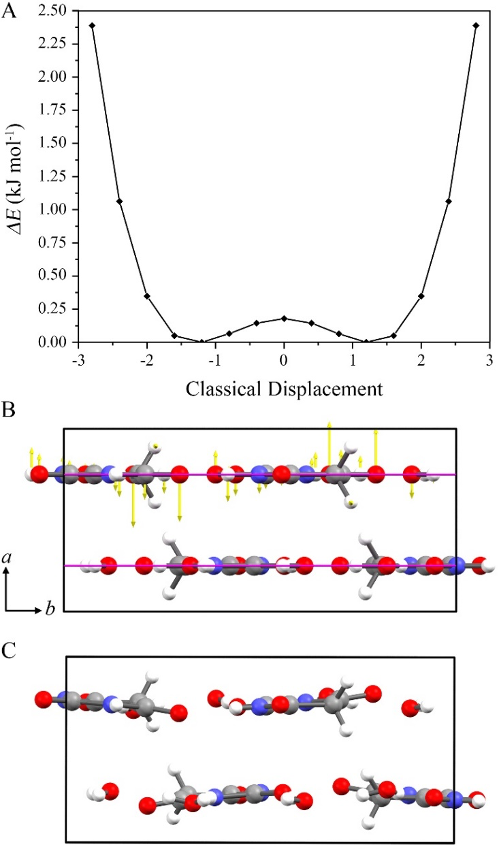
\includegraphics[width=7.5cm]{src/figures/btadh_figs/btadh_fig4.png}
  \caption{A) Scan of potential energy surface along the -35.79 cm\textsuperscript{-1} imaginary phonon mode (PBE/pob-TZVP) of BTADH confined to the \textit{Pnma} space group at 270-K lattice parameters. B) Displacement vectors (yellow arrows, magnitudes scaled ×10) for the imaginary mode shown for top two BTADH units. Displacements are oriented normal to the reflection plane (purple line) confining the molecules in \textit{Pnma} symmetry. C) Molecular orientation of BTADH optimized in \textit{P}2\textsubscript{1}/\textit{n} symmetry.}
  \label{doublewell}
\end{figure}
\newpage
\par Starting from the planar 270-K \textit{Pnma} crystal structure, symmetry constraints were removed and the geometry was re-optimized within fixed experimental X-ray lattice dimensions using PBE/pob-TZVP. The unit cell symmetry was relaxed to \textit{P}2\textsubscript{1}/\textit{n}, analogous to the suspected low-temperature phase, thus removing the reflection planes that confine the atoms in the \textit{Pnma} space group. From the optimized geometry, the measured molecular plane angles, as described in \autoref{btadh_planeorientations} and \autoref{btadh_latticeparams}, were 7.93°, 11.79°, and 36.82° corresponding to CH\textsubscript{2}–molecule, molecule–molecule, and H\textsubscript{2}O–H\textsubscript{2}O planes, respectively. These angles are remarkably similar to those observed for the X-ray crystal structures collected at low temperature. The relaxed-symmetry structural optimizations were repeated for each of the crystal dimensions measured at the 14 different temperatures in the range of 100–270 K using both the pob-TZVP and 6-311G(d,p) basis sets (\autoref{btadh_angles_table}). Analysis of the optimized geometries revealed little variation in measured angles over the temperature range. There was a general trend of angles increasing with decreasing temperature, but with no significant variations occurring between adjacent temperature steps.
An additional series of calculations were performed using the lattice dimensions of the suspected \textit{Pnma} phase, i.e. at temperatures above 217 K. The crystal structures were restricted to either \textit{P}2\textsubscript{1}/\textit{n} or \textit{Pnma} symmetry to evaluate differences in unit cell energies between the two crystal settings. In both basis sets, the \textit{P}2\textsubscript{1}/\textit{n}  symmetry produced the lower energy unit cell for all temperature lattice parameters (\autoref{E_pobtzvp}). The difference in energy between the \textit{P}2\textsubscript{1}/\textit{n} or \textit{Pnma} space groups were small in each case, ranging from -0.985 to -1.379 kJ mol-1 in the pob-TZVP basis, and -0.804 to -1.234 kJ mol\textsuperscript{-1} in 6-311G(d,p). These results show a slight energetic preference to \textit{P}2\textsubscript{1}/\textit{n} symmetry in unit cell dimensions at all temperatures above 216 K.

\begin{table}[htbp]
\centering
\tiny
\caption{Angles between the molecular planes of two molecules within the packed unit cell, angles between the two water molecules within the unit cell and the angles between the CH\textsubscript{2} plane and the molecular plane of one molecule.}
\begin{tabular}{cccccccccc}
\multicolumn{4}{c}{\textbf{CH\textsubscript{2}-Molecule\textsuperscript{a}(°)}} & \multicolumn{3}{c}{\textbf{Molecule-Molecule\textsuperscript{b} (°)}} & \multicolumn{3}{c}{\textbf{H\textsubscript{2}O-H\textsubscript{2}O\textsuperscript{c}(°)}} \\
\hline
& \textbf{pob-} & & & \textbf{pob-} & & & \textbf{pob-} \\
\textbf{T (K)} & \textbf{TZVP} & \textbf{6-311G(d,p)} & \textbf{exp.}  & \textbf{TZVP} & \textbf{6-311G(d,p)} & \textbf{exp.}  & \textbf{TZVP} & \textbf{6-311G(d,p)} & \textbf{exp.} \\
270 & 7.93 & 8.40 & --    &  11.79 & 11.27 & --     &  36.82 & 35.86 & -- \\
230 & 7.48 & 7.80 & --    &  11.19 & 10.55 & --     &  34.67 & 33.19 & -- \\
220 & 7.39 & 7.67 & --    &  11.07 & 10.41 & --     &  34.27 & 32.70 & -- \\
219 & 7.38 & 7.66 & --    &  11.12 & 10.43 & --     &  34.22 & 32.75 & -- \\
218 & 7.39 & 7.67 & --    &  11.14 & 10.45 & --     &  34.29 & 32.82 & -- \\
217 & 7.39 & 7.57 & --    &  10.88 & 10.19 & --     &  34.09 & 32.26 & -- \\
216 & 8.35 & 8.70 & 1.85  &  11.77 & 11.20 & 2.98   &  35.07 & 33.59 & 28.87 \\
215 & 8.34 & 8.63 & 2.47  &  11.57 & 10.95 & 2.97   &  34.65 & 32.86 & 8.85 \\
210 & 8.62 & 8.85 & 2.85  &  11.71 & 11.06 & 3.60   &  34.67 & 32.66 & 20.31 \\
200 & 9.12 & 9.39 & 3.72  &  12.25 & 11.70 & 5.11   &  35.20 & 33.53 & 26.94 \\
190 & 9.35 & 9.50 & 4.81  &  12.08 & 11.46 & 5.90   &  34.87 & 32.66 & 16.72 \\
170 & 9.65 & 9.79 & 5.80  &  12.17 & 11.56 & 7.18   &  34.53 & 32.07 & 20.06 \\
150 & 9.83 & 9.94 & 6.70  &  12.20 & 11.63 & 8.22   &  34.16 & 31.62 & 25.09 \\
100 & 10.05 & 10.02 & 8.14  & 12.06 & 11.44 & 9.96  & 33.22 & 30.19 & 27.36 \\
\hline
\multicolumn{10}{l}{\textsuperscript{a,b,c}Refer to Fig. 2 for plane definitions:  \textsuperscript{a}Fig. 2A; \textsuperscript{b}Fig. 2B; \textsuperscript{c}Fig. 2C.} \\
\label{btadh_angles_table}
\end{tabular}
\end{table}



\begin{table}[ht]
    \centering
    \begin{tabular}{ccc}
        \textbf{T(K)\textsuperscript{a}}    &   \textbf{\(\Delta\)E/pob-TZVP} &   \textbf{\(\Delta\)E/6-311G(d,p)}     \\
        \hline
        270     &   -1.379      &   -1.234          \\
        230     &   -1.116      &   -0.893          \\
        220     &   -1.050      &   -0.844          \\
        219     &   -1.050      &   -0.860          \\
        218     &   -1.050      &   -0.866          \\
        217     &   -0.985      &   -0.804          \\
        \hline
        \multicolumn{3}{l}{\textsuperscript{a}Lattice parameters for unit cells at variable}\\
        \multicolumn{3}{l}{temperatures are listed in \autoref{btadh_latticeparams}.}
    \end{tabular}
    \caption{Calculated energies (per BTA·2H\textsubscript{2}O) of BTADH confined to P2\textsubscript{1}/n and \textit{Pnma} symmetry groups at experimental lattice parameters. \(\Delta\)E provided in units of kJ mol\textsuperscript{-1}.}
    \label{E_pobtzvp}
\end{table}



THz vibrational frequencies were calculated for the low-temperature \textit{P}2\textsubscript{1}/\textit{n} phase using the fully relaxed unit cell structures (lattice dimensions provided in \autoref{btadh_latticeparams}) in PBE/pob-TZVP and PBE/6-311G(d,p) (\autoref{btadh_thz2}). The computed mode frequencies were mostly overestimated in comparison to the THz spectrum obtained at 78 K (\autoref{intensities}). This is typical in such calculations as the lattice dimensions used for normal mode calculations are contracted from the actual experimental dimensions due to neglect of thermal expansion in the DFT-optimized unit cells and contributions from basis set superposition error \citep{king_application_2011,king_modified_2012}. The result of constricting the unit cell dimensions is the general blue-shifting of vibrational frequencies as extensively shown in previous reports. In addition, vibrational anharmonicity of phonon modes contributes to overestimation of normal modes calculated in a harmonic limit \citep{ruggiero_resolving_2016,kleist_terahertz_2019,king_investigating_2010}. Frequencies were scaled by 0.80 in the spectral overlays provided in \autoref{btadh_thz2} to aid in visual comparison. Lorentzian lineshapes were convolved into calculated modes using the FWHM of the 33.6 cm\textsuperscript{-1} spectral feature to emphasize the large differences in linewidths observed in the THz spectrum. From the spectral simulations, the vibrational modes contributing to the observed THz absorptions can be assigned. A notable discrepancy between the phonon frequencies calculated by the two basis sets is the underestimation of the mode corresponding to the 33.6 cm\textsuperscript{-1} peak when using the 6-311G(d,p) basis set.

\begin{table}[ht]
    \centering
    \caption{Calculated phonon mode frequencies and intensities of full-relaxed BTADH unit cell in \textit{P}2\textsubscript{1}/\textit{n} symmetry using the PBE functional with the pob-TZVP and 6-311G(d,p) basis sets. }
    \begin{tabular}{c|c|c|c|c}
    \textbf{pob-TZVP} & \textbf{Int\textsuperscript{a}} & \textbf{6-311G(d,p)} & \textbf{Int} \\
    \hline
    43.46\textsuperscript{b} & 5.14 & 30.14 & 3.16 \\
    54.47 & 0.01 & 44.05 & 0.13 \\
    61.43 & 0.04 & 58.89 & 0.00 \\
    67.17 & 1.86 & 65.13 & 0.69 \\
    78.70 & 0.40 & 72.49 & 0.13 \\
    85.07 & 10.35 & 80.62 & 9.81 \\
    103.23 & 0.00 & 82.94 & 35.50 \\
    107.29 & 15.68 & 96.21 & 2.57 \\
    121.83 & 28.40 & 110.36 & 27.21 \\
    122.75 & 4.41 & 115.01 & 1.97 \\
    \hline
    \multicolumn{4}{l}{\textsuperscript{a}Intensity (km mol\textsuperscript{-1}); \textsuperscript{b}Frequency (cm\textsuperscript{-1})} \\

    \end{tabular}
    \label{intensities}
\end{table}
\newpage
\begin{figure}[h!]
  \center
  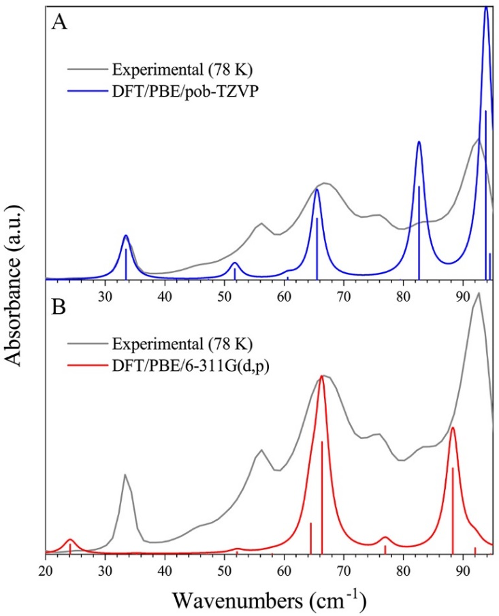
\includegraphics[width=10cm]{src/figures/btadh_figs/btadh_fig5.png}
  \caption{A) Mode character of the spectral feature at 33.6 cm\textsuperscript{-1} observed in the 78 K THz spectrum, represented by calculated displacement vectors (yellow arrows, magnitudes scaled ×10). B) Calculated mode displacements of the broad feature centered at 66.7 cm\textsuperscript{-1} in the 78 K THz spectrum. C) Mode character of the distinct 88.8 cm\textsuperscript{-1} vibrational mode observed in the 293 K THz spectrum (corresponding to the feature located at 92.7 cm\textsuperscript{-1} in the 78 K spectrum).}
  \label{btadh_thz2}
\end{figure}
\newpage
Of primary interest to explain the unexpected behavior of BTADH are the mode characters of the THz absorptions at 33.6, 66.7, and 92.1 cm\textsuperscript{-1}. The respective assignments of these modes were made by inspection of the spectral overlays, and are the 43.46, 85.07, and 121.83 cm\textsuperscript{-1} modes for PBE/pob-TZVP and the 30.14, 82.94, and 110.36 cm\textsuperscript{-1} modes for PBE/6-311G(d,p). Comparison of the vibrational motions for the assigned modes between the two basis sets confirms that these are indeed analogous modes. To reiterate the significance of these specific phonon vibrations, the 33.6 cm\textsuperscript{-1} mode appears in the THz spectrum at low temperature, but is ostensibly absent at room-temperature. The absorption at 66.7 cm\textsuperscript{-1} is unusually broad and is also not directly evident at room temperature. The 92.1 cm\textsuperscript{-1} mode, which is located at 88.8 cm\textsuperscript{-1} at room temperature, is present in the THz spectra at both 78 and 293 K and exhibits seemingly typical temperature-dependent phonon behavior. 
The calculated eigenvectors for each of the three normal modes are shown in \autoref{fig:btadh_vib_vectors}. It can be seen that the 33.6 and 66.7 cm\textsuperscript{-1} modes are along the direction of the suspected phase change relating the \textit{P}2\textsubscript{1}/\textit{n} and \textit{Pnma} symmetry cells perpendicular to the $\langle 100 \rangle$ lattice plane (\textit{P}2\textsubscript{1}/\textit{n} bc plane). The difference in the modes principally lies in the relative molecular translational and rotational contributions to each. The 33.6 cm\textsuperscript{-1} mode has primarily translational character with neighboring BTA molecules moving in opposing phase. The 66.7 cm\textsuperscript{-1} exhibits the adjacent BTA molecules rotating in-phase along the c-axis about their respective molecular centers of mass. In combination with the associated motions of the two H\textsubscript{2}O molecules, this vibration moves along a minima of the potential energy surface represented by the double-well potential shown in \autoref{doublewell}A relating two equivalent energetic minima. Finally, the vibrational mode corresponding the peaks at 88.8 and 92.7 cm\textsuperscript{-1} in the 293 K and 78 K spectra, respectively, consists of combined internal deformation of the BTA molecule, notably in the CH\textsubscript{2} groups, mixed with rotational character about the a-axis. The H\textsubscript{2}O molecular motions are both translational and rotational in character.

\begin{figure}[h!]
    \centering
    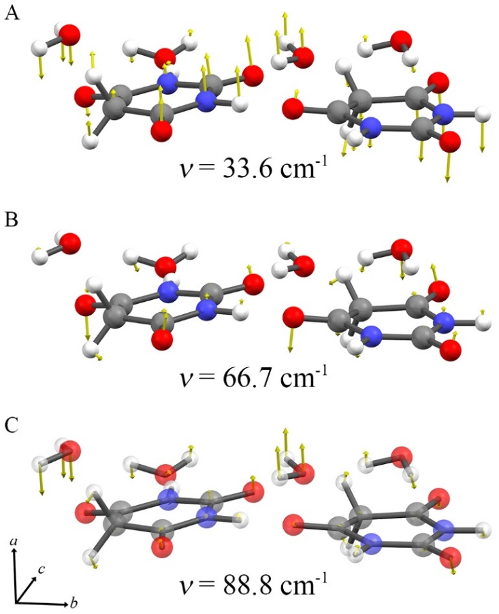
\includegraphics[width=0.5\linewidth]{src/figures/btadh_figs/btadh_fig6.png}
    \caption{(A) Mode character of the spectral features at 33.6 cm\textsuperscript{-1} observed in the 78 K THz spectrum, represented by calculated displacement vectors (yellow arrows, magnitudes scaled ×10). (B) Calculated mode displacements of the broad feature centered at 66.9 cm\textsuperscript{-1} in the 78 K THz spectrum. (C) Mode character of the distinct 88.8 cm\textsuperscript{-1} vibrational mode observed in the 293 K THz spectrum (corresponding to the feature located at 92.7 cm\textsuperscript{-1} in the 78 K spectrum).}
    \label{fig:btadh_vib_vectors}
\end{figure}

The unusual THz spectra obtained for BTADH can be explained by examining the vibrational mode characters. In the room-temperature spectrum, phonon modes having displacements primarily along the a-axis and are of rotational and translational character are not distinctly present, although a very broad absorption profile across the collection bandwidth is observed. The one distinct spectral feature at 293 K is due to a vibrational mode containing to a large extent intramolecular deformations, making it nearly independent of the barrier transition coordinate. We propose that subtle crystal disorder exists at higher temperatures about the low-energy barrier lying on the 〈100〉 lattice plane, or equivalently, the mirror plane confining the crystal system in imposed \textit{Pnma} symmetry. From our combined experimental and computational findings, the crystal system can more accurately be described in a monoclinic \textit{P}2\textsubscript{1}/\textit{n} setting having a \(\beta\) angle ~90°. Two degenerate energetic states exist in \textit{P}2\textsubscript{1}/\textit{n} related by a two-fold rotation about the b-axis, and the two states are separated by a low-energy barrier corresponding to the originally reported \textit{Pnma} structure. Given the quite low energy barrier as reported in \autoref{E_pobtzvp}, the crystal structure would be able to transition through the closely separated energy states, assuming there is sufficient thermal energy within the system. In this case, the resulting crystal structure would have the appearance of a time-averaged structure in a planar configuration that could be represented in \textit{Pnma} symmetry. 
Upon cooling below 217 K, the BTADH crystal structure settles into a \textit{P}2\textsubscript{1}/\textit{n} configuration. The degenerate energy states available for BTADH to access at higher temperatures provide the origins of the non-merohedral twinning phenomenon observed by X-ray diffraction in the system at reduced temperatures. The diminished thermal fluctuations in the crystal systems locks BTADH into either of the \textit{P}2\textsubscript{1}/\textit{n} configurations resulting in the possible twinning of neighboring unit cells joined about a two-fold b-axis rotation. Evidence of crystal twinning is also presented in the THz spectrum obtained at 78 K. Vibrational modes with motions in the direction of the transition coordinate connecting the two equivalent \textit{P}2\textsubscript{1}/\textit{n} structures, i.e. those which would pass through a near planar \textit{Pnma} structure with large atomic displacements, exhibit significant mode softening as these modes approach the transition state along their vibrational coordinates. Other similar vibrational modes that would not cross this planar structural barrier but do, however, have primary displacements perpendicular to the inversion plane appear in the THz spectrum collected at 78 K without significant broadening of spectral features. These same vibrational modes are not observed at 293 K as the modes are effectively washed out due to the subtle crystal disorder above 217 K.

\section{Conclusions}
Solid-state DFT and THz spectroscopy data suggest that at temperatures above the previously reported phase transition temperature of 217 K, the crystal does not exist in the \textit{Pnma} space group configuration. However, two equivalent energetic states with \textit{P}2\textsubscript{1}/\textit{n} symmetry lie on either side of the proposed \textit{Pnma} structure. It is these same minima that guide the crystal system to a non-merohedrally twinned configuration at decreased temperatures. At temperatures above 217 K, the system contains the thermal energy necessary to readily transition between these degenerate states separated by the nearly energetically equivalent \textit{Pnma} structural barrier. The spatial and energetic proximity of the \textit{P}2\textsubscript{1}/\textit{n} and \textit{Pnma} structures result in the subtle disorder of the BTADH system at higher temperatures. It is this disorder which initially led investigators through the comprehensive examination of the complexity in resolving what was thought to be a high-temperature phase, for which the \textit{Pnma} space group was settled despite remarkable efforts to define the system otherwise. The evidence presented in the current study point to an absence of a true temperature-dependent phase change, and rather to a system that exists in a delicately disordered state above the once-thought transition temperature.

\section{Acknowledgements}
We would like to acknowledge high-performance computing support of the R2 compute cluster (DOI: 10.18122/B2S41H) provided by Boise State University’s Research Computing Department. The Authors would like to thank Boise State University for continued support. 